%!TEX program = lualatex
\documentclass{report}
\usepackage[vietnamese]{babel}
\usepackage{hyperref}
\usepackage[acronym, toc]{glossaries}
\usepackage{graphicx}
\usepackage{fontspec}
\usepackage{titlesec}
\usepackage{fontsize}
\usepackage{xcolor}
\usepackage{caption}
\usepackage{subcaption}
\usepackage{float}
\usepackage{blindtext}
\usepackage{listingsutf8}
\usepackage{tikz}
\usepackage{fancyhdr}
\usepackage{indentfirst}

\changefontsize[20pt]{14pt}
\usepackage[
  paper=a4paper,
  left=30mm,
  right=20mm,
  top=25mm,
  bottom=25mm]{geometry}

\setmainfont{Times New Roman}

\titleformat{\chapter}[hang]
    {\normalfont\fontsize{16}{19}\bfseries}
    {Chương\ \thechapter:}
    {1em}
    {} 

\titleformat{\section}
    {\normalfont\fontsize{15}{19}\bfseries}
    {\thesection}
    {1em}
    {}
\titleformat{\subsection}
    {\normalfont\fontsize{14}{19}\bfseries\slshape}
    {\thesubsection}
    {1em}
    {}
\titleformat{\subsubsection}
    {\normalfont\fontsize{14}{19}\slshape}
    {\thesubsubsection}
    {1em}
    {}

\makenoidxglossaries

\newglossaryentry{latex}{
	name=Latex,
	description={Is a mark up language specially suited for scientific documents}
}

\newacronym{mcu}{VĐK}{vi điều khiển}
\newacronym{i2c}{I$^2$C}{Inter-Integrated Circuit}
\newacronym{uart}{UART}{Universal Asynchronous Receiver-Transmitter}
\newacronym{usart}{USART}{Universal Synchronous Asynchronous Receiver-Transmitter}
\newacronym{arm}{ARM}{Advanced RISC Machine}
\newacronym{usb}{USB}{Universal Serial Bus}
\newacronym{spi}{SPI}{Serial Peripheral Interface}
\newacronym{dma}{DMA}{Direct Memory Accecss}
\newacronym{adc}{ADC}{Analog to Digital Converter}

\lstset{basicstyle=\ttfamily, numbers=left, numberstyle=\small, numbersep=8pt, frame = single, breaklines=true}

\pagestyle{fancy}
\renewcommand{\chaptermark}[1]{\markboth{#1}{#1}}
\fancyhead[R]{}
\fancyhead[L]{\leftmark}

\widowpenalties 1 10000
\raggedbottom

\begin{document}

\begin{titlepage}
	
	\begin{center}
		\begin{tikzpicture}[remember picture,overlay,inner sep=0,outer sep=0]
		     \draw[blue!70!black,line width=4pt]
		     ([xshift=-1.5cm,yshift=-2cm]current page.north east) coordinate (A)--
		     ([xshift=2.5cm,yshift=-2cm]current page.north west) coordinate(B)--
		     ([xshift=2.5cm,yshift=2cm]current page.south west) coordinate (C)--
		     ([xshift=-1.5cm,yshift=2cm]current page.south east) coordinate(D)--
		     cycle;
		\end{tikzpicture}
		
		\textbf{HỌC VIỆN KỸ THUẬT MẬT MÃ}
		
		KHOA CÔNG NGHỆ THÔNG TIN
		
		\vspace{1cm}
		
		
\includegraphics[width=0.3\textwidth]{../images/kma.png}
		
		
		\vspace{2.2cm}
		
		\textbf{BÀI TẬP MÔN LẬP TRÌNH DRIVER}
		
		\vspace{0.2cm}
		
		\color{red}
		\textbf{LẬP TRÌNH DRIVER I2C CHO MÀN HÌNH LCD 1602 TRÊN LINUX}
		
		
		
	\end{center}

	\begin{flushleft}        
		\hspace{3cm}
		Khoa: Công nghệ thông tin
		
		\hspace{3cm}
		Chuyên ngành: Kỹ thuật phần mềm nhúng và di động
		
		
		\vfill
		
		\hspace{3cm}
		
		\hspace{3cm}Người hướng dẫn
		
		\begin{tabular}{l c}
			
			\hspace{4cm}\textbf{Giảng viên: Triệu Vũ Anh Quân} \\
			
			
		\end{tabular}
		
		\vspace{0.5cm}
		
		\hspace{3cm}Nhóm sinh viên thực hiện:
		
		\begin{tabular}{l c c}
			
			\hspace{4cm}Phạm Văn Dũng & CT040308 \\
						
			\hspace{4cm}Phạm Thị Phương Anh & CT040401 \\
			
			\hspace{4cm}Lại Phương Thảo & CT040445 \\
						
			\hspace{4cm}Cao Văn Giáp & CT030317\\
			
			\hspace{4cm}Nhóm 02
			
			
		\end{tabular}
		
	\end{flushleft}
	
	\begin{center}
		
		\vspace{1cm}
		
		Hà Nội - 2023
		
	\end{center}
\end{titlepage}

\pagenumbering{arabic}

\chapter{GIỚI THIỆU CÔNG CỤ}
\section{Màn hình LCD1602 HD44780}
\paragraph{}
Màn hình LCD1602 là màn hình ma trận điểm với 2 hàng, mỗi hàng chứa 16 ký tự kích thước 5x8 điểm. HD44780 là một IC điều khiển màn hình ma trận 5x8 hoặc 5x10 với tối đa 80 ký tự, phù hợp với màn hình LCD1602. Việc điều khiển yêu cầu tối thiểu 6 chân GPIO. Các bước khởi tạo màn hình.


\begin{figure}[H]
	\centering
	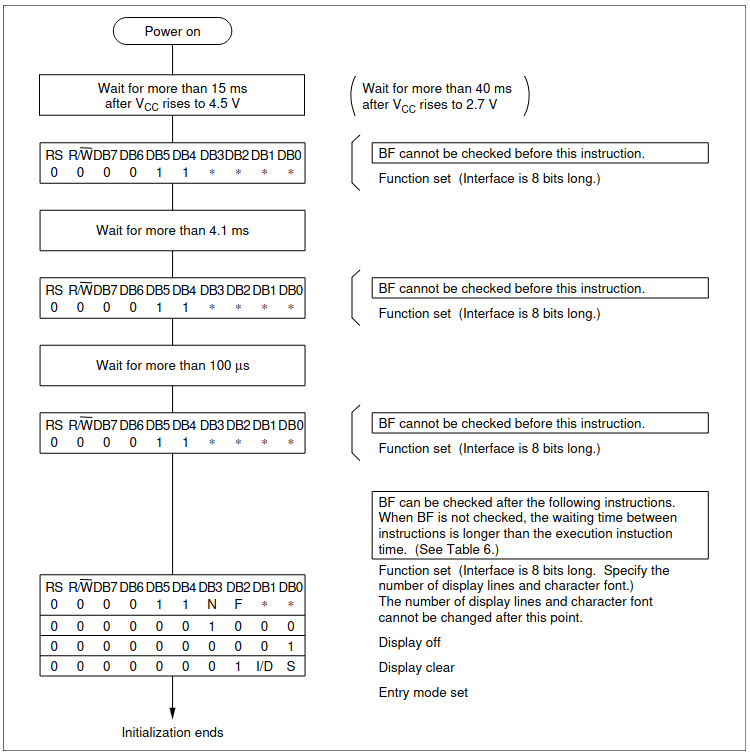
\includegraphics[width=0.6\textwidth]{images/hd44780_init.png}
	\caption{Khởi tạo HD44780}
\end{figure}
\section{Module mở rộng GPIO PCF8574 cho LCD1602}

I2C là một chuẩn được phát triển bởi Philips. Nó là một giao thức 2 dây chậm với tốc độ có thể lên đến 400 kHz. Nó được sử dụng rộng rãi trong hệ thống nhúng. Một số thiết bị sử dụng biến thể không đạt được yêu cầu của I2C nên có thể được gọi bằng tên khác như TWI hoặc IIC.

SMBus (System Management Bus) dựa trên giao thức I2C được sử dụng rộng rãi trong hệ thống máy tính. Rất nhiều thiết bị I2C có thể hoạt động trên SMBus như I2C EEPROMs và một số chip theo dõi phần cứng.

Trong một bus I2C, có thể có một hay nhiều master chip được kết nối tới một hay nhiều slave chip.


\begin{figure}[H]
	\centering
	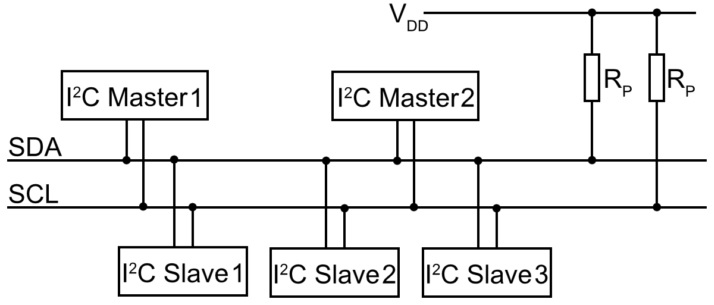
\includegraphics[width=0.6\textwidth]{../images/I2C-Bus-Layout.jpg}
	\caption{I2C bus}
\end{figure}


Master chip là thiết bị kết nối tới slave. Trong nhân linux, master chip được gọi là một adapter hoặc bus. Các trình điều khiển của adapter nằm trong thư mục con drivers/i2c/busses.

Một algorithm chứa mã có thể sử dụng để cài đặt nhiều loại I2C adapter. Mỗi adapter driver có thể phụ thuộc vào một algorithm driver trong thư mục con drivers/i2c/algos hoặc chứa mã cho riêng nó.

Một slave chip là nút thực hiện giao tiếp khi có yêu cầu của master. trong Linux, nó được gọi là client. Client driver được lưu trong thư mục nào phụ thuộc vào các chức năng mà nó cung cấp, ví dụ như trong drivers/media/gpio cho thiết bị mở rộng GPIO.

\paragraph{}
Để đơn giản hóa việc điều khiển một thiết bị sử dụng nhiều GPIO, module mở rộng chân sử dụng kết nối nối tiếp sẽ giúp đơn giản hóa việc kết nối và tiết kiệm số chân GPIO. PCF8574 sử dụng giao tiếp I2C có 8 địa chỉ có thể thay đổi cứng. Địa chỉ mặc định là 0x27 và có 8 chân GPIO song song. Việc đọc 8 chân GPIO có thể thực hiện bằng việc đọc 8 bit từ module PCF8574, tương tự, ghi vào 8 chân GPIO được thực hiện bằng việc ghi 8 bit tương ứng.

\section{Phát triển \acrshort{i2c} device driver}
\paragraph{}
Linux kernel driver là một module được nạp vào nhân linux và chạy trên không gian địa chỉ của nhân linux giúp cung cấp các chức năng mở rộng cho nhân hệ điều hành.
\paragraph{}
Device driver trong linux là một kernel module cung cấp giao diện giao tiếp với các thiết bị phần cứng như USB, PCI, I2C, SPI, … Device driver thực hiện việc giao tiếp như gửi và nhận dữ liệu, từ thiết bị, đảm bảo cho thiết bị được hoạt động đúng mục đích đặt ra.
\paragraph{}
Khác với các thiết bị như PCI hay USB, thiết bị sử dụng giao tiếp I2C mặc định không được nhận biết bởi phần cứng mà thay vào đó phần mềm phải nhận biết những thiết bị nào được kết nối ở địa chỉ nào. Có một số cách để thực hiện việc này nhưng một phương pháp hiệu quả là sử dụng Device tree.
\paragraph{}
Device tree là một cấu trúc dsữ liệu và một hệ thống mô tả phần cứng được sử dụng trong hệ điều hành linux. Trong Device tree, các thiết bị I2C được khai báo tại bus và địa chỉ xác định. Cùng với thông tin bus và địa chỉ, Device tree còn mô tả loại driver tương thích với thiết bị. Khi trình điều khiển thiết bị được nạp, hàm probe sẽ được gọi khi trình điều khiển tương thích với thiết bị được khai báo trong Device tree.
\paragraph{}
Một Device tree cho thiết bị slave I2C có cấu trúc dạng như sau: thiết bị i2c-device được kết nối tới i2c-bus có địa chỉ 0x50. Driver tương thích là “vendor,i2c-device":
\begin{lstlisting}
	i2c {
		compatible = "i2c-bus";
		#address-cells = <1>;
		#size-cells = <0>;
		i2c-device@50 {
			compatible = "vendor,i2c-device";
			reg = <0x50>;
		}
	}
\end{lstlisting}
\paragraph{}
Bên trong driver, sau khi hàm probe được gọi với tham số struct i2c\_client tương ứng, thực hiện lưu lại biến này để thực hiện giao tiếp với thiết bị. Để đọc từ i2c device, sử dụng hàm i2c\_smbus\_read*, và i2c\_smbus\_write* cho việc ghi.


\section {Giao tiếp với device driver}

Một số lựa chọn để giao tiếp với device driver của thiết bị nhúng bao gồm:

\begin{itemize}
	\item Sử dụng Character device driver
	\item Sử dụng sysfs
	\item Kết hợp các phương pháp
\end{itemize}
	

Với character device driver thiết bị được xuất hiện trên không gian người dùng với một file duy nhất bên trong /dev. Các thao tác có thể được thực hiện thông qua các lời gọi từ struct file\_operations như open, close, read, write, ioctl. Thông qua device file, thiết bị dạng vào/ra sẽ đơn giản hơn thông qua các lời gọi hệ thống. Một số ứng dụng sử dụng device file bao gồm: Giao tiếp với cổng serial, đọc từ ổ đĩa, …

Khác với character device driver, ứng dụng có thể sử dụng sysfs cho việc thiết lập và quản lý cấu hình. Các file trong không gian người dùng xuất hiện dưới dạng thư mục trong /sys/kernel/. Bên trong thư mục này là các file cấu hình được tạo ra với device driver giúp chương trình trong không gian người dùng có thể tương tác với driver thông qua việc đọc ghi các file. Giao tiếp với thiết bị phần cứng sẽ dễ dàng hơn thông qua sysfs do phần cứng có nhiều tham số cần đọc và ghi và chúng được tách riêng chúng ra từng file.

Với phần cứng hỗ trợ cả cấu hình các tham số và vào ra lượng thông tin lớn, kết hợp cả character device driver và sysfs sẽ tận dụng được lợi thế của cả hai phương pháp. Các thao tác vào ra sẽ được thực hiện qua character device driver, các thao tác cấu hình sẽ được thực hiện thông qua hệ thống sysfs và thao tác ioctl của character device driver. Khi đó người dùng có thể làm quen với thiết bị thông qua sysfs và thực hiện các thao tác qua chúng. Khi lập trình, việc sử dụng character device driver sẽ đem lại hiệu quả cao hơn.

\chapter{THIẾT KẾ DRIVER}

Driver được triển khai trên nhiều file. File lcd\_data.h chứa dữ liệu cho hoạt động điều khiển của driver (nội dung hiển thị, các dữ liệu điều khiển hiển thị, cuộn trang, ...).  File lcd\_sysfs.h giúp xuất dữ liệu driver và thay đổi dữ liệu driver theo yêu cầu của người dùng sử dụng hệ thống sysfs. File lcd\_i2c\_client.h chứa các hàm tương tác với thiết bị như điều khiển đèn nền, điều khiển cuộn trang hay thay đổi dữ liệu. File pcf\_lcd.c là file chính của driver, thực hiện khai báo driver, khởi tạo luồng điều khiển, các hàm probe, remove.

\begin{figure}[H]
	\centering
	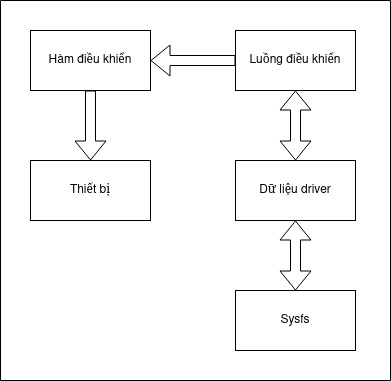
\includegraphics[width=0.8\textwidth]{../images/driver.jpg}
	\caption{Sơ đồ khối driver}
\end{figure}
Trong luồng điều khiển hoạt động của driver, thực hiện liên tục lấy dữ liệu hiển thị cho màn hình. Dữ liệu này có thể thay đổi sau mỗi lần lặp do dữ liệu mới được cập nhật hoặc sau khi làm mới dữ liệu, ở chế độ cuộn văn bản, dữ liệu hiển thị bị dịch chuyển sang ký tự khác. Sơ đố luồng điều khiển được thể hiện trong hình \ref{f:work-thread}.
\begin{figure}[H]
	\centering
	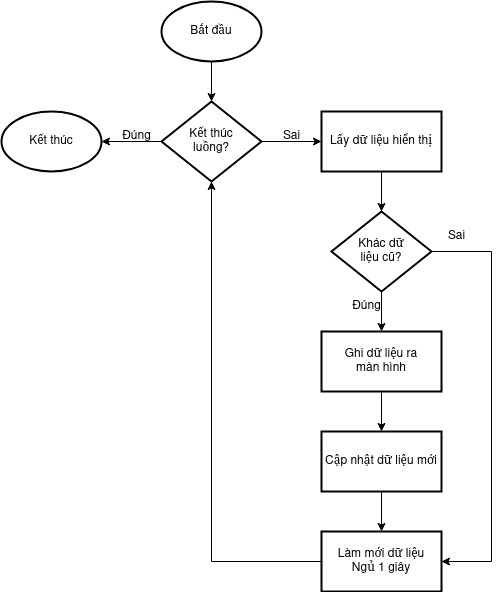
\includegraphics[width=0.8\textwidth]{../images/driver-work-thread.jpg}
	\caption{Luồng điều khiển}
	\label{f:work-thread}
\end{figure}

Khi khai báo driver, thực hiện tạo đối tượng struct i2c\_driver trong đó bao gồm các trường probe\_new cho việc khởi tại thiết bị, .remove cho việc 	gỡ bỏ thiết bị, .id\_table là đối tượng struct i2c\_device\_id cho thiết bị, .of\_match\_table là struct of\_device\_id chứa thông tin tên thiết bị tương thích với driver được lưu trong device tree.
\lstinputlisting[firstline=66, firstnumber=66, lastline=109]{../../pcf_lcd.c}

Việc làm mới dữ liệu được thực hiện liên tục để phục vụ mục đích hiển thị dữ liệu mới từ người dùng hoặc phục vụ mục đích cuộn nội dung. Hàm làm mới dữ liệu được khai báo bên trong file chứa dữ liệu.
\lstinputlisting[firstline=8,firstnumber=8, lastline=23]{../../lcd_data.h}
\lstinputlisting[firstline=143,firstnumber=143, lastline=176]{../../lcd_data.h}

\chapter{THIẾT KẾ GIAO DIỆN}
Để giúp việc điều khiển thiết bị được đơn giản hơn, nhóm thực hiện thiết kế một giao diện đơn giản dựa trên QT. Các thao tác trên giao diện là được thực hiện tương ứng với giao diện trong sysfs của driver.

\begin{figure}[H]
	\centering
	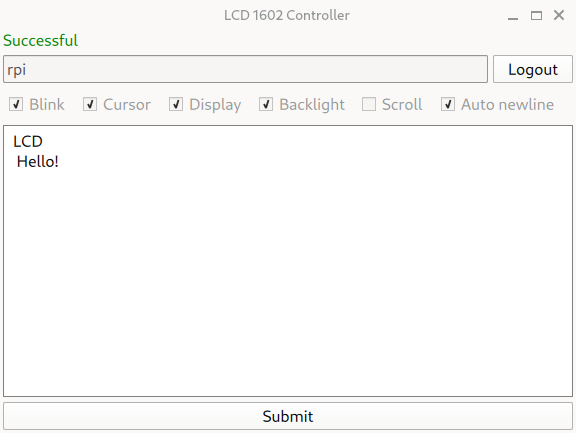
\includegraphics[width=0.8\textwidth]{../images/gui.png}
	\caption{Giao diện đồ họa cho thiết bị}
\end{figure}


\end{document}
